\documentclass[UTF8]{ctexart}
\usepackage{graphicx}
\usepackage{subfigure}
\usepackage{float}
\title{第一次技术文档}
\author{刘畅 15061183}

\begin{document}
	\maketitle
	% \tableofcontents
	\section{程序说明}
	\noindent
	\textbf{使用语言:} JAVA \newline
	\textbf{编程环境:} Windows 8.1 + Eclipse Neon.3 Release (4.6.3) \newline
	\textbf{程序结构:} \newline
	\indent \textbf{ImageProcessor 类} \newline
	\indent void grayscale(String filename, String outputLabel) \{..\} // 输出灰度化后图片 \newline
	\indent void histogramCorrection(String filename, String outputLabel, int partNum) \{..\} // 输出直方图均衡处理后图片 \newline
	\indent void globalStretch(String filename, String outputLabel, int lowerScale, int upperScale) \{..\} // 输出全局灰度线性拉伸(压缩)处理后图片 \newline
	\indent void localStretch(String filename, String outputLabel, int oriLowerScale, int oriUpperScale, int lowerScale, int upperScale) \{..\} // 输出局部灰度线性拉伸(压缩)处理后图片 \newline
	\indent int[][] getGreyMatrix(BufferedImage image) \{..\} // 获取图片的灰度矩阵 \newline
	\indent int[] getGreyCounts(int[][] greyMatrix) \{..\} // 根据灰度矩阵,统计各灰度像素数 \newline
	\indent int[] getGreyTransMap(int[] greyCounts, int partNum) \{..\} // 建立灰度映射表 \newline
	\indent int[][] transGrey(int[][] oriGreyMatrix, int[] greyTransMap) \{..\} // 根据灰度映射表,转化灰度矩阵 \newline
	\indent BufferedImage getHist(int[] values) \{..\} // 根据灰度像素数,获取灰度直方图 \newline
	\indent BufferedImage getGreyImage(int[][] greyMatrix) \{..\} // 根据灰度矩阵,获取灰度图 \newline
	\indent void outputImage(String filename, String type, BufferedImage image) \{..\} // 输出图片 \newline

	\section{准备工作:图片灰度化}
		\subsection{实现过程}
			\subsubsection{灰度矩阵的获取}
			在对一个宽度为$w$、高度为$h$图片进行\textbf{直方图均衡}和\textbf{灰度线性拉伸}处理之前,需要先对图像进行灰度化处理。假设某像素灰度级为$Y$,根据像素的$R$、$G$、$B$值利用公式
			\[ Y=0.3R+0.59G+0.11B \]
			将每个点的灰度级$Y$记录在灰度矩阵$M(w,h)$中。
			\subsubsection{输出灰度图}
			根据灰度矩阵$M(w,h)$,建立一个宽度为$w$,高度为$h$的新图片,并将图片上任意一个像素点的$R$、$G$、$B$值都设定为$M(w,h)$中对应位置的灰度级$Y$,保证图片各个像素点$R$、$G$、$B$值相等。该图即为原图的灰度图。
		\subsection{处理效果}

		\begin{figure}[H]
		\centering
		\subfigure[原彩色图]{
			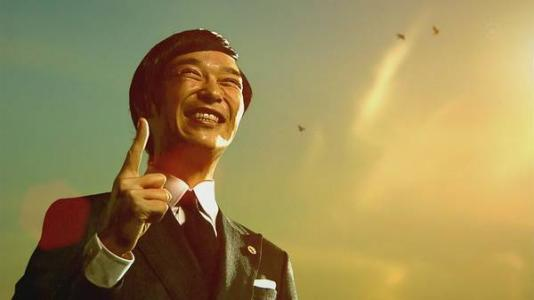
\includegraphics[width=0.48\textwidth]{lh_color.jpg}}
		\subfigure[处理后灰度图]{
			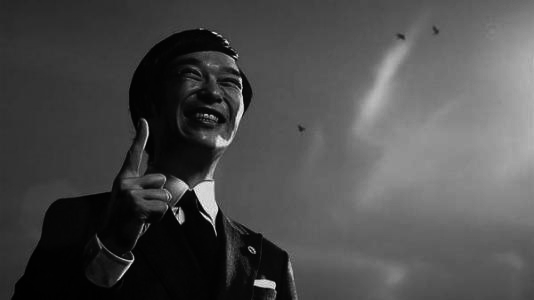
\includegraphics[width=0.48\textwidth]{lh_grey.png}}
		\caption{灰度处理效果}
		\end{figure}


	\section{任务一:直方图均衡}
		\subsection{算法实现}
		根据读取图像得到的灰度矩阵$M(w,h)$,可以计算出第$i$种灰度所占的像素数量$n_i$。假设灰度级为$L$(在该程序中,取$L=256$),则第$k$个灰度级均衡变换后的新灰度级$s_k$可由以下公式得到:
		\[ s_k=(L-1)\sum_{i=0}^k\frac{n_i}{wh} \]

		\subsection{处理效果}
			\subsubsection{图片一}
			\begin{figure}[H]
			\centering
			\subfigure[原灰度图]{
				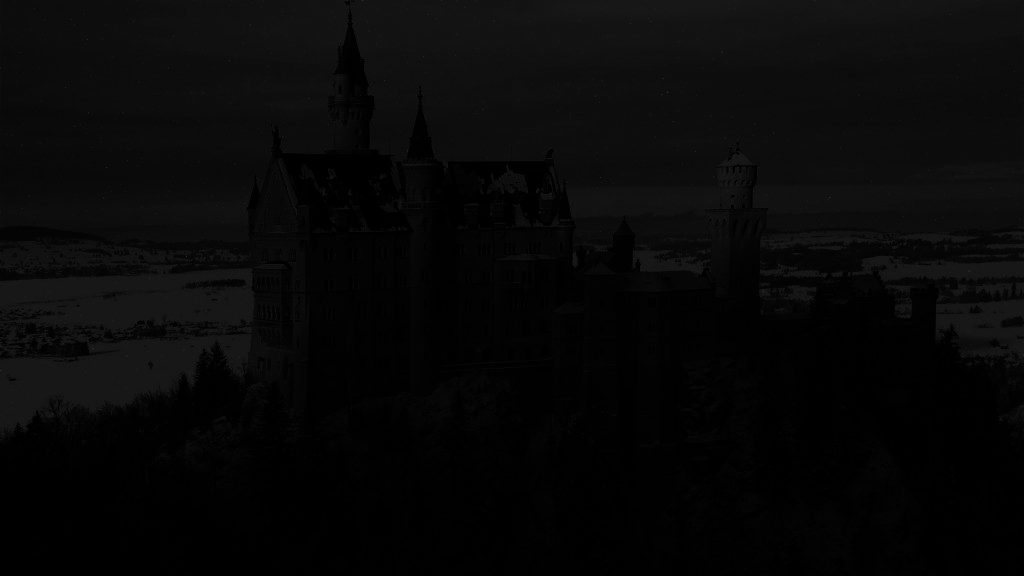
\includegraphics[width=0.48\textwidth]{cas_grey.png}}
			\subfigure[均衡处理后灰度图]{
				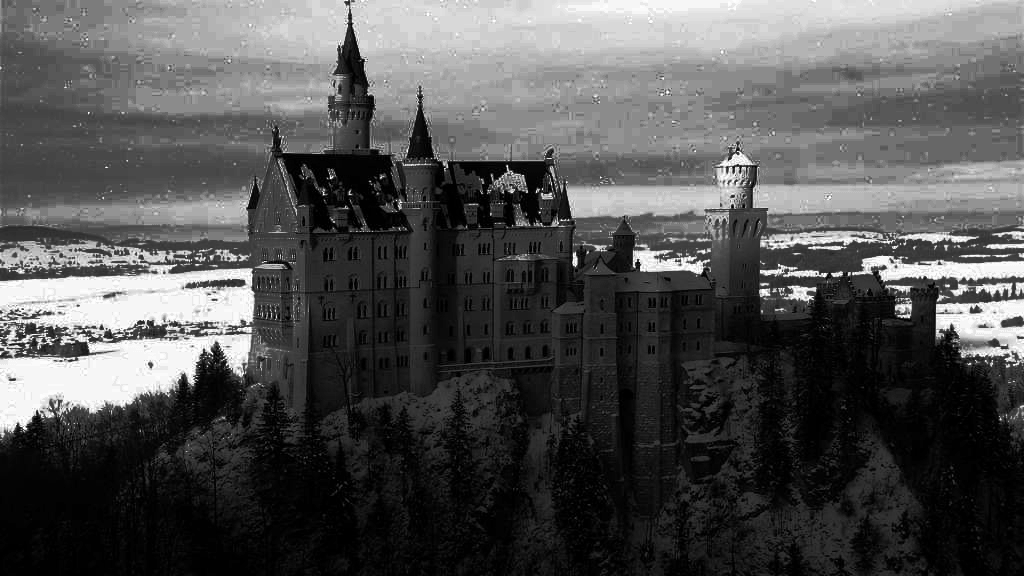
\includegraphics[width=0.48\textwidth]{cas_cor_1.png}}
			\subfigure[原灰度分布]{
				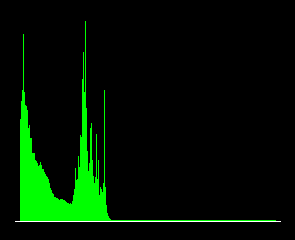
\includegraphics[width=0.48\textwidth]{cas_grey_hist.png}}
			\subfigure[均衡处理后灰度分布]{
				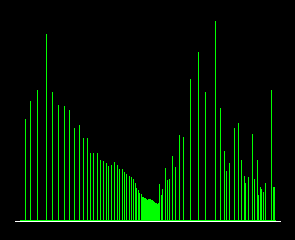
\includegraphics[width=0.48\textwidth]{cas_cor_1_hist.png}}
				\caption{图片二直方图均衡效果}
			\end{figure}

			可以看到,整体偏暗的城堡画面经过直方图均衡处理后变得清晰许多,直方图也的确变得更分散了,这符合算法的预期。

			\subsubsection{图片二}
			\begin{figure}[H]
			\centering
			\subfigure[原灰度图]{
				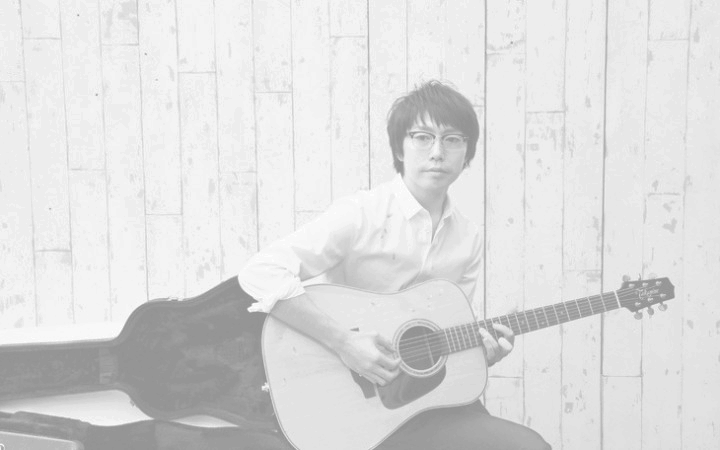
\includegraphics[width=0.48\textwidth]{yuu_grey.png}}
			\subfigure[均衡处理后灰度图]{
				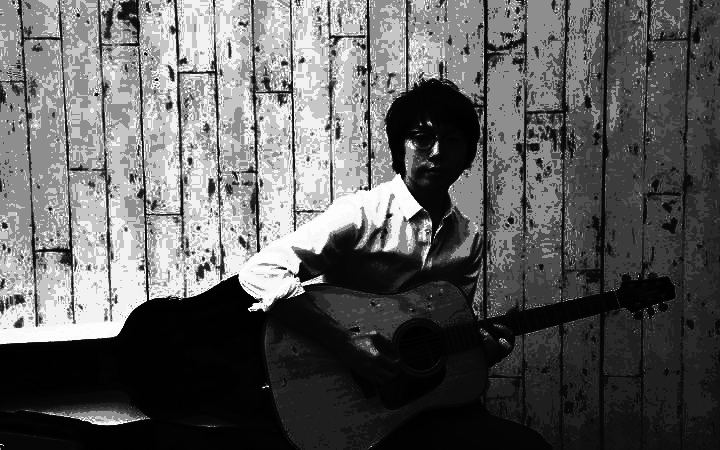
\includegraphics[width=0.48\textwidth]{yuu_cor_1.png}}
			\subfigure[原灰度分布]{
				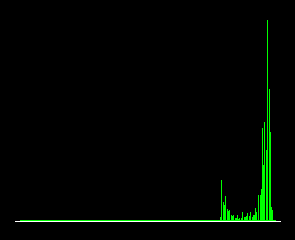
\includegraphics[width=0.48\textwidth]{yuu_grey_hist.png}}
			\subfigure[均衡处理后灰度分布]{
				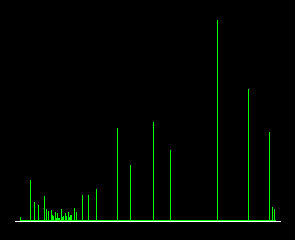
\includegraphics[width=0.48\textwidth]{yuu_cor_1_hist.png}}
				\caption{图片二直方图均衡效果}
			\end{figure}

			但是在图片二中,直方图均衡的结果虽然正确,但其效果并不理想,主要体现在均衡结果中人物部分的灰度级过高,以至于看不清具体细节。下面我对直方图均衡算法进行了一点改进,起到一定的优化效果。


		\subsection{改进}
			\subsubsection{算法}
			从图8中可以看到,效果不理想的主要原因是图片整体灰度级较低,而图片中人物的灰度级相较偏高,导致均衡后灰度级大大上升。为了解决大量低灰度对高灰度的干扰,我尝试将处理前的灰度级进行分段操作,如低灰度区和高灰度区,然后在这两部分分别进行直方图均衡处理,避免了低灰度区对高灰度区的干扰。\newline
			\indent 假设灰度的分段数为$p$,首先采用以下公式计算出平均每段的像素数$n_{avg}$:
			\[ n_{avg} = \frac{wh}{p} \]
			之后,根据$n_avg$对灰度级由低至高进行分段,尽可能保证每段内像素数总和相等。假设第$k$个灰度级所处段的最低灰度级为$r_{min}$,最高灰度级为$r_{max}$,则其均衡变换后的新灰度级$s_k$可由以下公式得到:
		\[ s_k=r_{min}+(r_{max}-r_{min})\sum_{i=r_{min}}^k\frac{n_i}{\sum_{j=r_{min}}^kn_j} \]


		 	\subsubsection{效果}

			\begin{figure}[H]
			\centering
			\subfigure[直方图均衡后灰度图(p=1)]{
				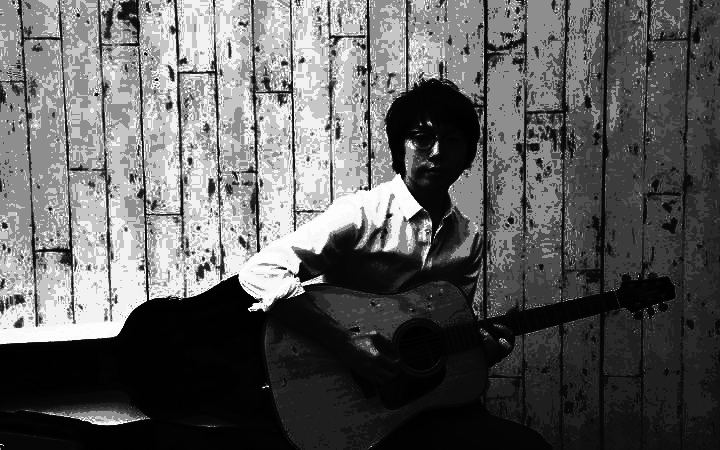
\includegraphics[width=0.48\textwidth]{yuu_cor_1.png}}
			\subfigure[直方图均衡后灰度图(p=2)]{
				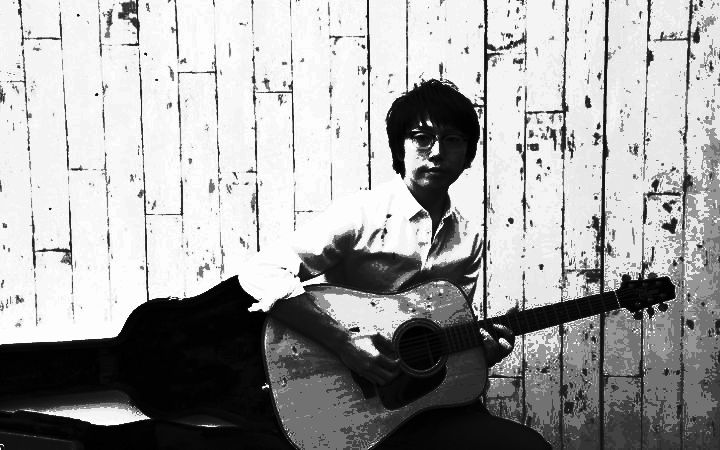
\includegraphics[width=0.48\textwidth]{yuu_cor_2.png}}
			\subfigure[直方图均衡后灰度图(p=3)]{
				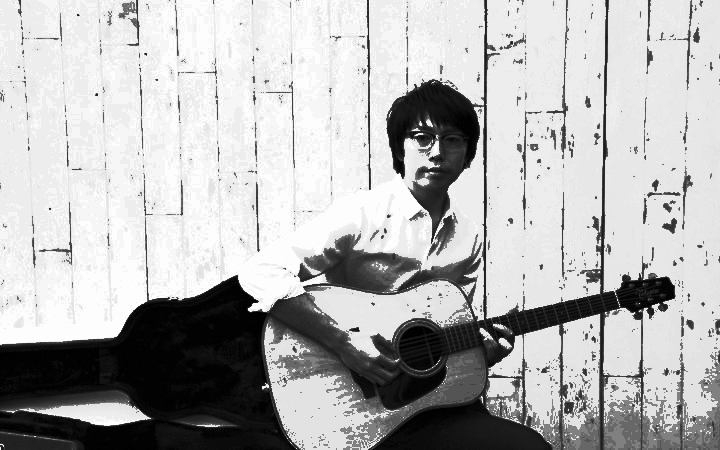
\includegraphics[width=0.48\textwidth]{yuu_cor_3.png}}
			\subfigure[直方图均衡后灰度图(p=4)]{
				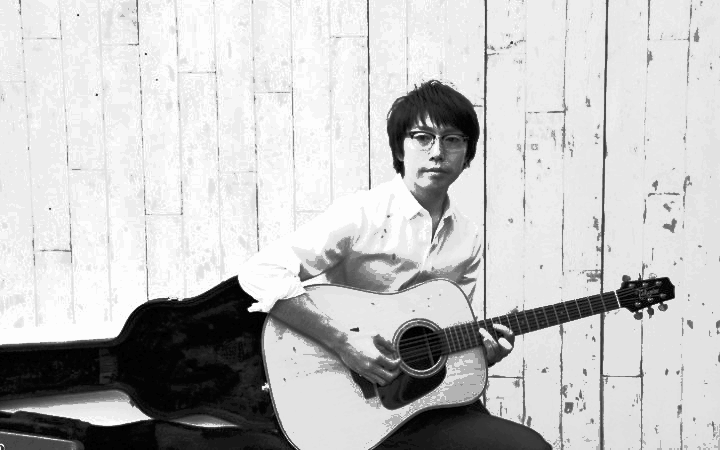
\includegraphics[width=0.48\textwidth]{yuu_cor_4.png}}
			\subfigure[直方图均衡后灰度图(p=5)]{
				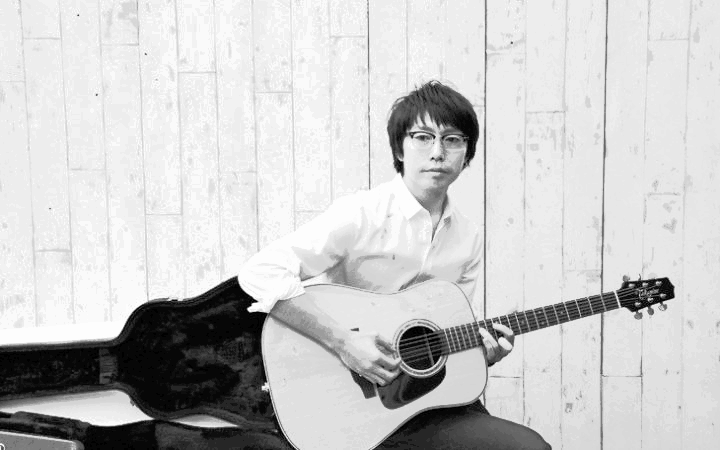
\includegraphics[width=0.48\textwidth]{yuu_cor_5.png}}
			\subfigure[原灰度图]{
				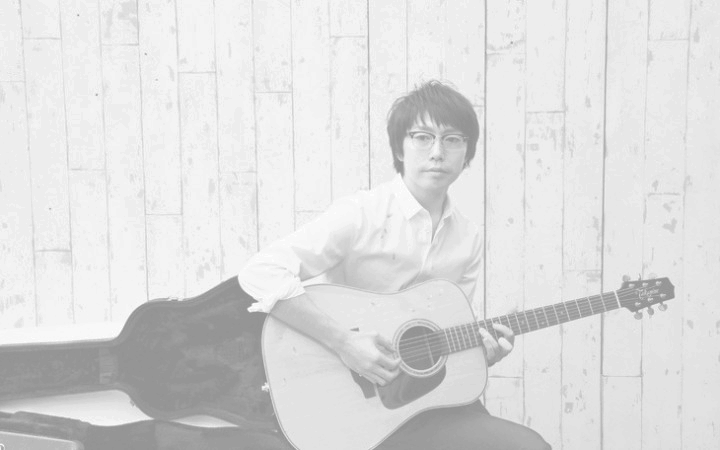
\includegraphics[width=0.48\textwidth]{yuu_grey.png}}
				\caption{直方图均衡优化处理后灰度图效果}
			\end{figure}


			\begin{figure}[H]
			\centering
			\subfigure[直方图均衡后直方图(p=1)]{
				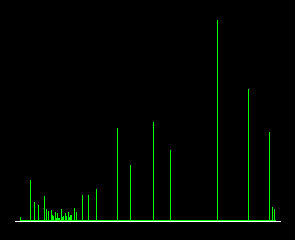
\includegraphics[width=0.48\textwidth]{yuu_cor_1_hist.png}}
			\subfigure[直方图均衡后直方图(p=2)]{
				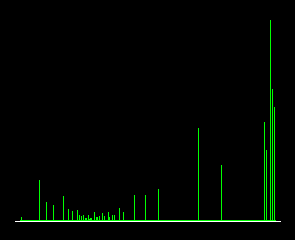
\includegraphics[width=0.48\textwidth]{yuu_cor_2_hist.png}}
			\subfigure[直方图均衡后直方图(p=3)]{
				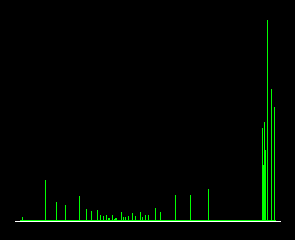
\includegraphics[width=0.48\textwidth]{yuu_cor_3_hist.png}}
			\subfigure[直方图均衡后直方图(p=4)]{
				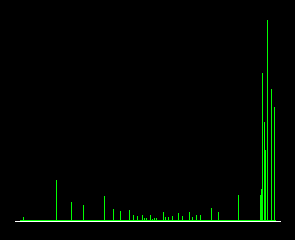
\includegraphics[width=0.48\textwidth]{yuu_cor_4_hist.png}}
			\subfigure[直方图均衡后直方图(p=5)]{
				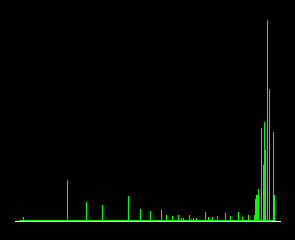
\includegraphics[width=0.48\textwidth]{yuu_cor_5_hist.png}}
			\subfigure[原直方图]{
				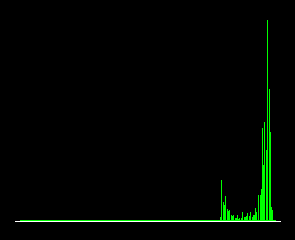
\includegraphics[width=0.48\textwidth]{yuu_grey_hist.png}}
				\caption{直方图均衡优化处理后灰度分布}
			\end{figure}

			从结果可以发现,随着分段数$p$的增大,均衡后的灰度图越来越接近于原图;随着$p$的减小,均衡后的灰度图越来越接近于优化前的均衡灰度图($p=1$)。就效果而言,取$p=4$与$p=5$的均衡灰度图效果优于前三幅,说明这种优化是合理的。\newline
			\indent但这并不代表着对于所有图片,取$p=4$与$p=5$结果都为最好,比如在用图片一进行分段的时候,发现还是取$p=1$即不优化的效果最好,说明$p$的最终取值还要由不同图片的性质决定。

		\subsection{总结}




	\section{任务二:灰度线性拉伸(压缩)}
		\subsection{算法实现}
		\subsection{处理效果}
			\subsubsection{全局拉伸(压缩)}
			\subsubsection{局部拉伸(压缩)}
		\subsection{总结}
	\section{比较与总结}
\end{document}

